\subsection{Estudo geométrico}
O estudo geométrico é uma avaliação simples de alcance dos manipuladores
industriais no ambiente do aro câmara. Tem como objetivo verificar se o
manipulador consegue percorrer todos os pontos da pá dentro das restrições da
tarefa HVOF, assumindo a pá planar, e diferentes posições de base. O estudo
leva em consideração as seguintes posições para o manipulador: escotilha
superior e base móvel; manipulador em frente à pá e base móvel verticalmente;
manipulador entre as pás e base móvel verticalmente.

Assumimos $R = 3.95 m$ e $R_m = 3 m$, onde $R$ é a distância do centro do cone à
superfície do aro câmara, e $R_m$ é o comprimento da pá. Logo, podemos
inferir o comprimento do aro câmara $P = 2*\pi *R = 24.81 m$. Em relação ao
centro do cone, o setor circular que cada pá ocupa tem um ângulo, em radianos,
de $\alpha = \frac{R_m*2*\pi}{P} = 0.76$, e a metade do setor circular entre
as pás tem ângulo $\beta = \pi/4$, já que elas são simetricamente distribuídas.
A figura~\ref{pa} mostra os parâmetros acima, onde as pás estão representadas
como setores circulares roxos e metade da distância entre as pás como setor
azul.

\begin{figure}[h!]
\centering
	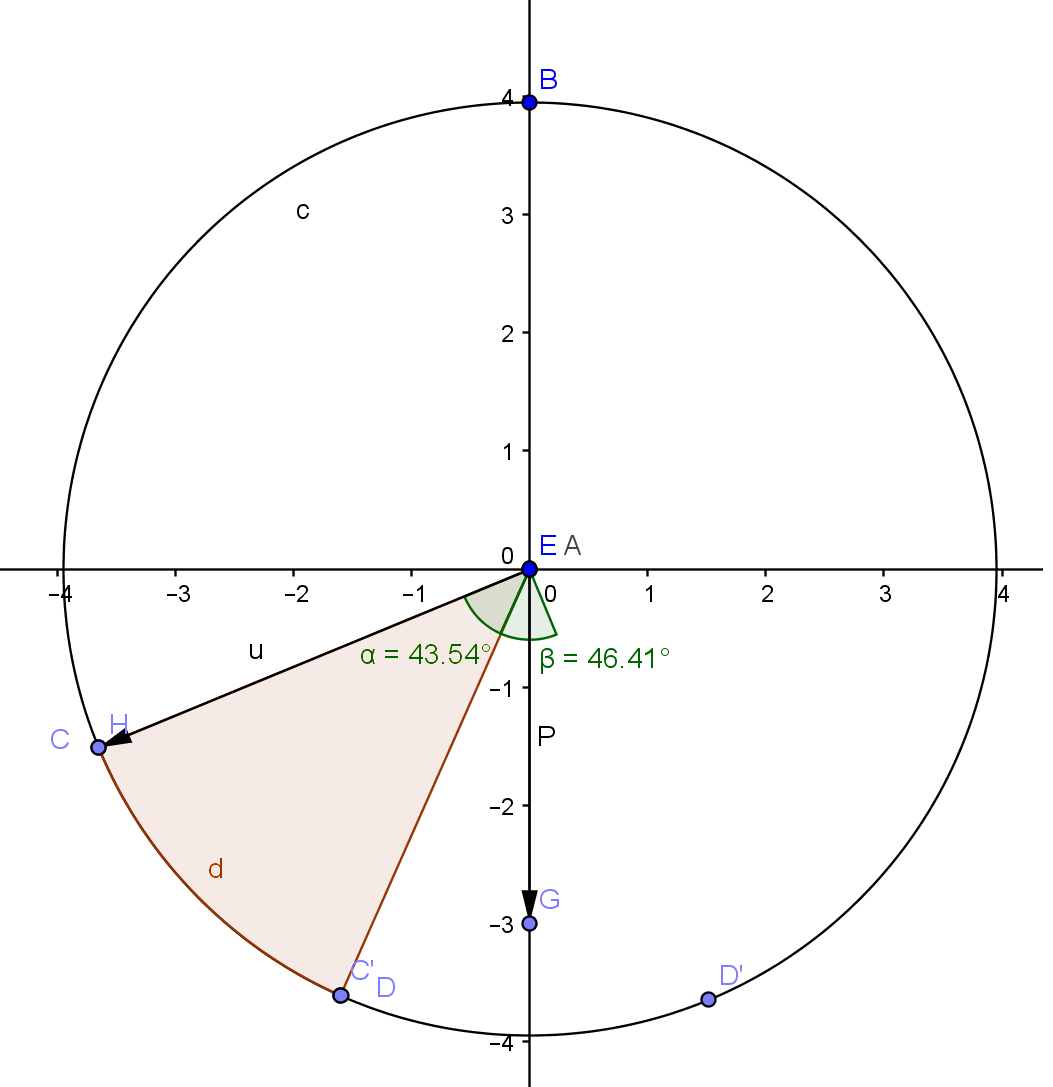
\includegraphics[width=\columnwidth]{figs/estudo/geometrico/pa.png} 
	\caption{Parâmetros do aro câmara.}
	\label{pa}
\end{figure}

Utilizando notação vetorial, temos: $\overrightarrow{P_1} = (0,-R,0)$. Considere
$$\overrightarrow{{P_2}} = R_z(-(\alpha/2 + \beta))
\overrightarrow{P_1}$$ e $$\overrightarrow{{P_3}} = R_z(-\beta))
\overrightarrow{P_1}$$ , onde $R_z$ é rotação em  torno de $Z$. Considere agora
o vetor $$\overrightarrow{d} =
R_{\overrightarrow{\overline{P_3}}}(-\omega)R_z(-\alpha/2 -
\beta)\overrightarrow{P_1}$$, onde $R_{\overrightarrow{\overline{P_3}}}$ é rotação em torno do vetor unitário
na direção de $\overrightarrow{P_3}$ e $\omega$ é o ângulo de rotação da pá em
seu próprio eixo (valor que pode variar de $0$ a $28^o$).
Dessa forma, busca-se o $$min (\left \| \overrightarrow{d} - \overrightarrow{M} 
\right \|) =\left \| R_{\overrightarrow{\overline{P_3}}}(-\omega)R_z(-\alpha/2 -
\beta)\overrightarrow{P} - \overrightarrow{M} \right \|$$, onde
$\overrightarrow{M}=(0,-x,0)$ é a localização da base do manipulador. Dessa
forma, obtemos a menor distância entre base e o extremo da pá para $\omega,
x, \beta$. Consequentemente, pode-se inferir o alcance mínimo do manipulador.

Pode-se posicionar a base do manipulador em diferentes valores de $\beta$, que é
o mesmo que girar a turbina e alterar a posição da pá. Para $\beta = 0$, por
exemplo, o manipulador se encontra em frente à pá, e para $\beta = \pi/4$ ele está entre as pás.

A análise para a escotilha inferior consiste em posicionar o manipulador no
centro ou entre as pás ($\beta = 0$ ou $\beta = \pi/4$). \ldots 

Na escotilha superior, como há restrição em relação ao manipulador (LBR 820), há
a necessidade de base móvel, que pode assumir diversos comprimentos e posições.
A solução de uma base com dois elos está representada na figura~\ref{pakuka},
onde os elos i e j estão representados em verde, o cone representado pela
circunferência c, o espaço de trabalho planar do manipulador está representado
em verde, 

\begin{figure}[h!]
\centering
	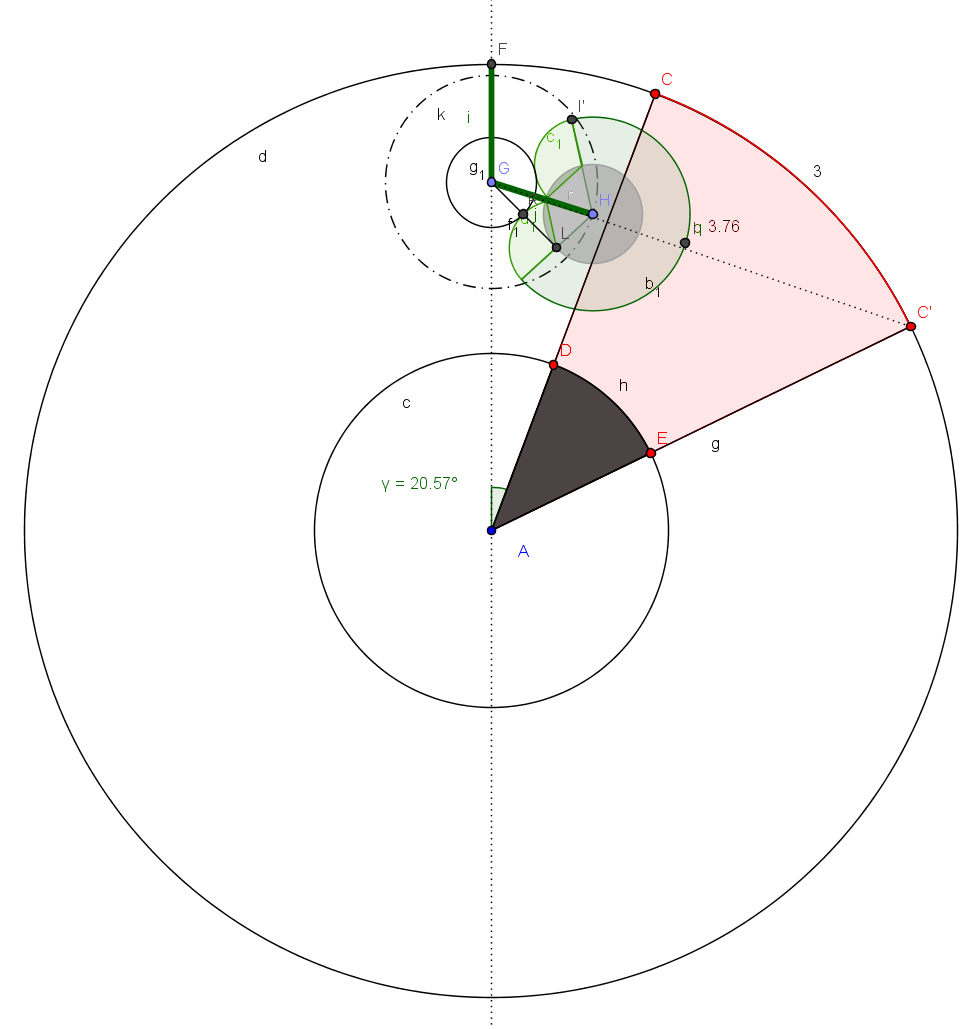
\includegraphics[width=\columnwidth]{figs/estudo/geometrico/kuka.png} 
	\caption{Estudo geométrico do manipulador industrial Kuka 820 na escotilha
	superior e base de dois elos.}
	\label{pakuka}
\end{figure}

A análise puramente geométrica não considera o formato real curvilíneo da pá e
é apenas uma análise de alcance de extremos. Isso não garante que a área de
trabalho do manipulador cubra todos os pontos da pá e ainda não considera
possíveis colisões com o ambiente e/ou própria base e manipulador. O estudo do
espaço de trabalho por simulações se faz necessário para garantir a viabilidade
dos manipuladores industriais.
